 \documentclass[11pt]{article}
\usepackage[finnish]{babel}
\usepackage[utf8]{inputenc}
\usepackage{graphicx}
\usepackage{float}
\usepackage{epstopdf}
\usepackage{tikz}
\usepackage[nottoc]{tocbibind}
\definecolor{sininen}{HTML}{CCE6FF}
\definecolor{vihrea}{HTML}{CCFFCC}
\definecolor{keltainen}{HTML}{FFEFCC}
\definecolor{punainen}{HTML}{FFC0CB}
\definecolor{purppura}{rgb}{0.90, 0.80, 1.00}
\definecolor{turkoosi}{rgb}{0.80, 1.00, 0.90}
\definecolor{limetti}{rgb}{0.90, 1.00, 0.80}
\definecolor{persikka}{rgb}{1.00, 0.90, 0.80}
\renewcommand*{\familydefault}{\sfdefault}
\title{\textbf{Keskustelufoorumi}\\ \small{dokumentaatio}}
\author{John Lång\\ \small{jllang@cs.helsinki.fi}}
\date{22.6.2014}
\begin{document}

\pagestyle{empty}
\maketitle
\thispagestyle{empty}

\newpage
\tableofcontents

\newpage
\thispagestyle{plain}

\section{Johdanto}
	Tämän projektin tarkoituksena on toteuttaa perinteinen web-pohjainen keskus-telufoorumi. Ohjelmiston
	avulla internetin käyttäjät voivat perustaa omia (yleen-sä tiettyyn aihepiiriin keskittyviä) yhteisöjään,
	joihin jokainen rekisteröity jäsen voi tuottaa omaa, ensisijaisesti tekstuaalista, sisältöään. Lisäksi
	projektin tavoitteena on luonnollisesti tarjota mahdollisimman tehokkaat ja käyttäjäystävälliset työkalut
	foorumin ylläpidosta sekä moderoinnista vastaaville yhteisön jäsenille, jotta he voisivat suorittaa
	tehtäväänsä tarkoituksenmukaisesti.
		
	Aion toteuttaa projektin käyttämällä Java-ohjelmointikieltä Netbeans IDE:llä sekä  PostgreSQL-tietokantaa 
	ja Apache Tomcat -http-palvelinta. Loppukäyttä-jälle näkyvän sivuston ulkoasun aion toteuttaa HTML 5- sekä
	mahdollisesti CSS-kielten avulla. HTML-koodin generoimiseen käytän JSP-, Unified EL-, ja JSTL- tekniikoita.
	Versionhallintaan käytän Git:iä sekä GitHub-palvelua.
	%Tavoitteenani on myös salata mahdollisimman suuri osa foorumin tietoliikenteestä HTTPS-protokollan avulla.
	%Foorumin yleiset asetukset tallennetaan XML-tiedostoihin.
	
	Itse tämän dokumentin laatimisessa olen käyttänyt hyväkseni avoimen lähde-koodin ohjelmistoja.
	Gummi:lla olen tehnyt itse PDF-tiedoston (käyttäen tekstin latomiseen maineikasta \LaTeX-jäjrestelmää),
	Dialla kaaviot, LibreOffice Calc:lla käyttötapausmallin sekä tietokohteiden taulukot, sekä Inkscapella
	muuttanut nämä kuvat EPS-formaattiin PDF-tiedostoon liittämistä varten. Lisäksi eräiden kuvien käsittelyssä
	olen käyttänyt GIMP-ohjelmaa.
	
	Pyrkimyksenäni on pitää järjestelmän vaatima asennustyö minimissä enkä siksi aio käyttää muita kun kielten
	standardikirjastoja sekä mainitsemiani palve-linohjelmistoja. Poikkeuksia äskeiseen olen tehnyt 
	kryptografisen tiivistefunktion osalta, jota käytän salasanojen suojaamiseen, sekä CSS-väriliukujen osal-ta.
	Tiivisteen laskemista en ole keksinyt itse, vaan käytän siihen \emph{PBKDF2}-nimistä menetelmää \cite{a}.
	Värilukujen tuottamiseen puolestaan olen käyttänyt internetissä olevaa generaattoria \cite{b}.	Lisäksi
	aion tehdä ohjelmistostani	mahdollisimman näkymättömän loppukäyttäjälle siten, ettei foorumin käyttäminen
	edellytä mitään selainliitännäisiä tai Javascriptin käyttöä. Luultavasti joudun kuitenkin (valitettavasti) 
	käyttämään evästeitä esimerkiksi käyttäjäkohtaisten istunto- ja	asetustietojen tallentamiseen.
	
	Olen valinnut projektilleni MIT-lisenssin, joka löytyy juurihakemiston tiedostosta LICENCE.
	% Tämän voisi varmaan mainita myös README.md:ssä
	
%	Haluan vielä esittää pahoitteluni kirjainten huonosta ladonnasta LibreOfficella tehdyissä taulukoissa.
%	(Jostain syystä kirjaimet eivät mene PDF:ksi muuntaessa oikein paikoileen, toisin kuin tulostaessa.)
%	Myös kaavioeditori näyttää hieman bugittaneen ER-kaavion parin viivan kanssa.
\newpage
\thispagestyle{plain}

\section{Yleiskuva}
	\subsection{Keskustelufoorumi}
		Keskustelufoorumi koostuu erilaisista lomakkeista ja työkaluista, joiden avulla järjestelmän tilaa
		muokataan, sekä tasopohjaisesta pääsynvalvonnasta neljällä eri \emph{käyttäjätasolla}.\footnote{
		Myöhemmin saatan ehkä lisätä myös käyttäjäryhmät, joiden perusteella voitaisiin valvoa
		pääsyä eri keskustelualueille saman kategorian käyttäjätunnusten keskuudessa.}
	
	\subsection{Käyttäjätasot}
		% Mitäpä jos olisi sellainen "puheoikeudeton" käyttäjätaso jonka käyttäjät saisivata vain käyttää
		% hakutoimintoja?
		Käyttäjätasot ovat \emph{vierailija}, \emph{jäsen}, \emph{moderaattori} ja \emph{ylläpitäjä}.
		Tasoihin liittyvät käyttöoikeudet ovat sisäkkäisiä siten, että vierailijalla on kaikkein suppeimmat
		ja ylläpitäjällä laajimmat käyttöoikeudet. Toisin sanoen ylläpitäjän oikeuksiin sisältyy kaikkien
		muiden tasojen oikeudet. Ylläpitäjä on keskustelufoorumin käyttöönoton suorittava henkilö. Alla on
		Vennin kaavio käyttäjätasoista.
	
		\begin{figure}[H]
			\vspace{1cm}
			\centering
			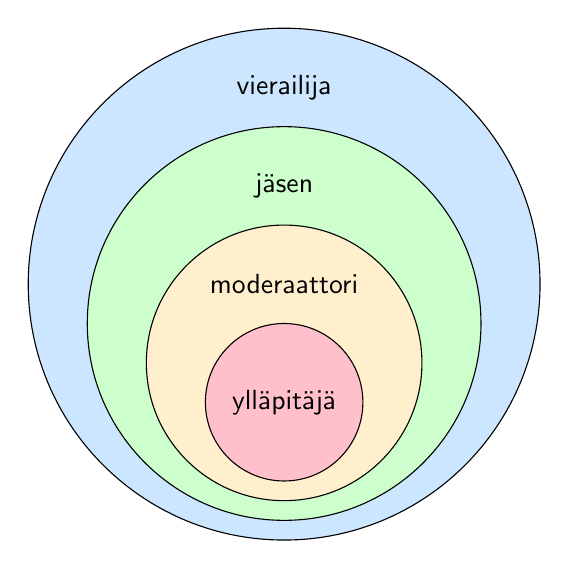
\begin{tikzpicture}
				\draw[fill=sininen] (0,1.5) circle(3.25);
				\draw[fill=vihrea] (0,1) circle(2.5);
				\draw[fill=keltainen] (0,0.5) circle(1.75);
				\draw[fill=punainen] circle(1);
				\node at (0,0) {ylläpitäjä};
				\node at (0,1.5) {moderaattori};
				\node at (0,2.75) {jäsen};
				\node at (0,4) {vierailija};
			\end{tikzpicture}\\
			\caption{Käyttäjätasot}
		\end{figure}
	
	\newpage
	\thispagestyle{plain}
	\subsection{Rakenne ja toiminnot}
		Foorumin toiminnallisuuden ytimessä ovat käyttäjien tuottamaa sisältöä säilövät
		\emph{ketjut}\footnote{Käytän ketjusta myös synonyymiä \emph{viestiketju}.}, jotka
		sijaitsevat \emph{keskustelualueilla}. Lähtökohtaisesti kuka tahansa kes-kustelufoorumin web-sivustolla
		surffaava käyttäjä eli vierailija voi \emph{selata} keskuste-lualueita ja lukea niissä olevien ketjujen
		\emph{viestejä}.\footnote{
		Tavoitteenani on luoda ensin vain litteä hierarkia sisältäen yhden tasoisia keskustelualueita,
		joissa on vierailijoille näkyviä tavallisia ketjuja. Jos aikaa jää, saatan myös toteuttaa esimerkiksi
		sisäkkäisiä ja vierailijoilta piilotettuja keskustelualueita.}
		Lisäksi vierailija voi rekis-teröidä itselleen käyttäjätunnuksen.	
	
		\begin{figure}[H]
			\centering
			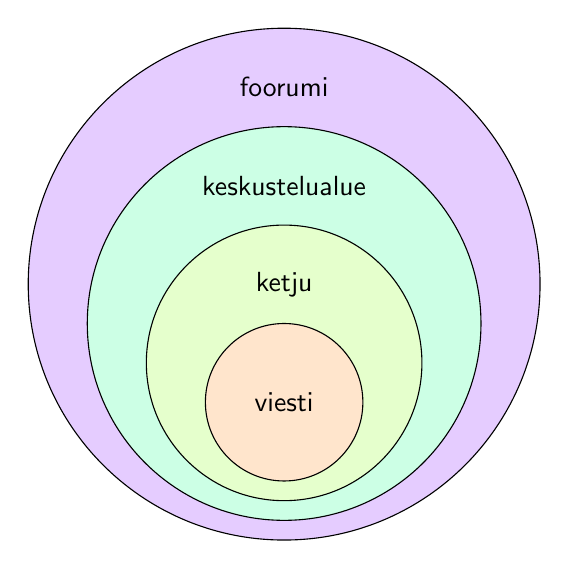
\begin{tikzpicture}
				\draw[fill=purppura] (0,1.5) circle(3.25);
				\draw[fill=turkoosi] (0,1) circle(2.5);
				\draw[fill=limetti] (0,0.5) circle(1.75);
				\draw[fill=persikka] circle(1);
				\node at (0,0) {viesti};
				\node at (0,1.5) {ketju};
				\node at (0,2.75) {keskustelualue};
				\node at (0,4) {foorumi};
			\end{tikzpicture}\\
			\caption{Foorumin rakenne}
		\end{figure}
	
		Jokainen rekisteröity käyttäjä eli jäsen voi aloittaa uuden ketjun sekä lisätä, muokata ja poistaa
		omia viestejään lukitsemattomissa ketjuissa. Näistä operaa-tioista käytän yhteisesti ilmausta
		\emph{viestitoiminnot}. Viestitoimintojen lisäksi jäse-net voivat käyttää \emph{hakutoimintoa}
		ketjujen ja viestien etsimiseen sekä muokata muille näytettäviä tietoja \emph{käyttäjätunnustoiminnoissa}. On syytä huomata että jäsentason käyttöoikeudet siis liittyvät
		\emph{käyttäjätunnuksiin} eli niiden käyttö edellyttää \emph{sisäänkirjautumista}.
	
		Moderaattorit ovat laajemmilla oikeuksilla toimivia
		käyttäjiä jotka voivat käsitellä mitä tahansa ketjun viestiä sekä lukita ja avata ketjun taikka siirtää
		sen toiselle keskustelualueelle.\footnote{Näin alkuvaiheessa en aio luvata mitään hienompia
		ominaisuuksia, kuten esimerkiksi ketjun määrittäminen \emph{tiedotteeksi} (joka saisi ketjun näkymään
		keskustelualueen listauksessa ennen tavallisia ketjuja).}
		Näistä toiminnoista käytän nimitystä \emph{moderointi}.
		\newpage
		\thispagestyle{plain}
		\noindent
		Moderaattorien toimenkuvana on pitää huolta siitä että ketjujen ja viestien sisäl-tö vastaa foorumin
		tarkoitusta.\footnote{Foorumin tarkoitutksesta päättää ylläpitäjä ja siten asia on projektini
		aihealueen ulkopuolella.}
		Moderoinnin lisäksi moderaattoreilla on oikeus antaa \emph{porttikieltoja} jäsenille. Porttikiellot
		estävät sisäänkirjautumisen ja kohdistuvat käyttäjätunnuksiin (ei esimerkiksi IP-osoitteisiin, sillä
		niiden estäminen ei ole tehokasta ja voi haitata sivullisia).
	
		Viimeinen käyttäjätaso on ylläpitäjä. Ylläpitäjät voivat poistaa käyttäjätun-nuksen sekä korottaa taikka
		alentaa sen tasoa. Näissä toiminnoissa on kyse \emph{käyttäjätunnusten hallinnasta}. Lisäksi ylläpitäjä
		voi \emph{hallita keskustelualueita} eli perustaa, muokata tai poistaa keskustelualueen.
	
	\subsection{Käyttötapaukset}
		Edellä esitettyä vastaa seuraava käyttötapauskaavio:
		\begin{figure}[H]
			\centering
			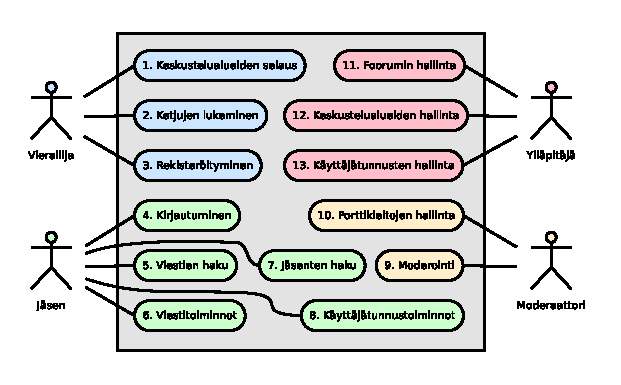
\includegraphics[trim = 7mm 0mm 0mm 0mm,scale=1.5]{kayttotapauskaavio.eps}\\
			\caption{Käyttötapauskaavio}
		\end{figure}
	
		Luettelen sivuilla 9-17 maineikasta Alistair Cockburnin käyttötapausmallia \cite{c}
		vapaasti mukaillen ohjelmistoni tärkeimmät käyttötapaukset.
	
		\newpage
		\thispagestyle{plain}
		\noindent
		Selkeyden vuoksi olen käyttänyt taulukoissa samaa värikoodauta kuin käyttö-tapauskaavioissa erottamaan
		eri käyttäjätasojen käyttötapaukset. Olen myös merkinnyt tähdellä (*) ne käyttötapausten vaiheet,
		jotka ovat valinnaisia. Valinnaisen vaiheen voi jättää kokonaan tekemättä. Jos valinnainen vaihe
		sisältää syötteen antamista, niin käyttäjä voi antaa tyhjän syötteen. Jos valinnainen vaihe ohitetaan,
		ei siltä osin muuteta tietokannassa olemassaolevia tietoja. (Toi-saalta tyhjä syöte tyhjentää jonkin
		kentän arvon sitä vastaavassa tietokannan monikon attribuutissa ja merkitsee siten eri asiaa kuin
		vaiheen ohittaminen).\footnote{Lisähuomioina mainittakoon, että käyttötapaus 2 on suunnittelun
		myöhemmässä vaiheessa siirretty vierailijalta jäsenelle.}
	
		\newpage
		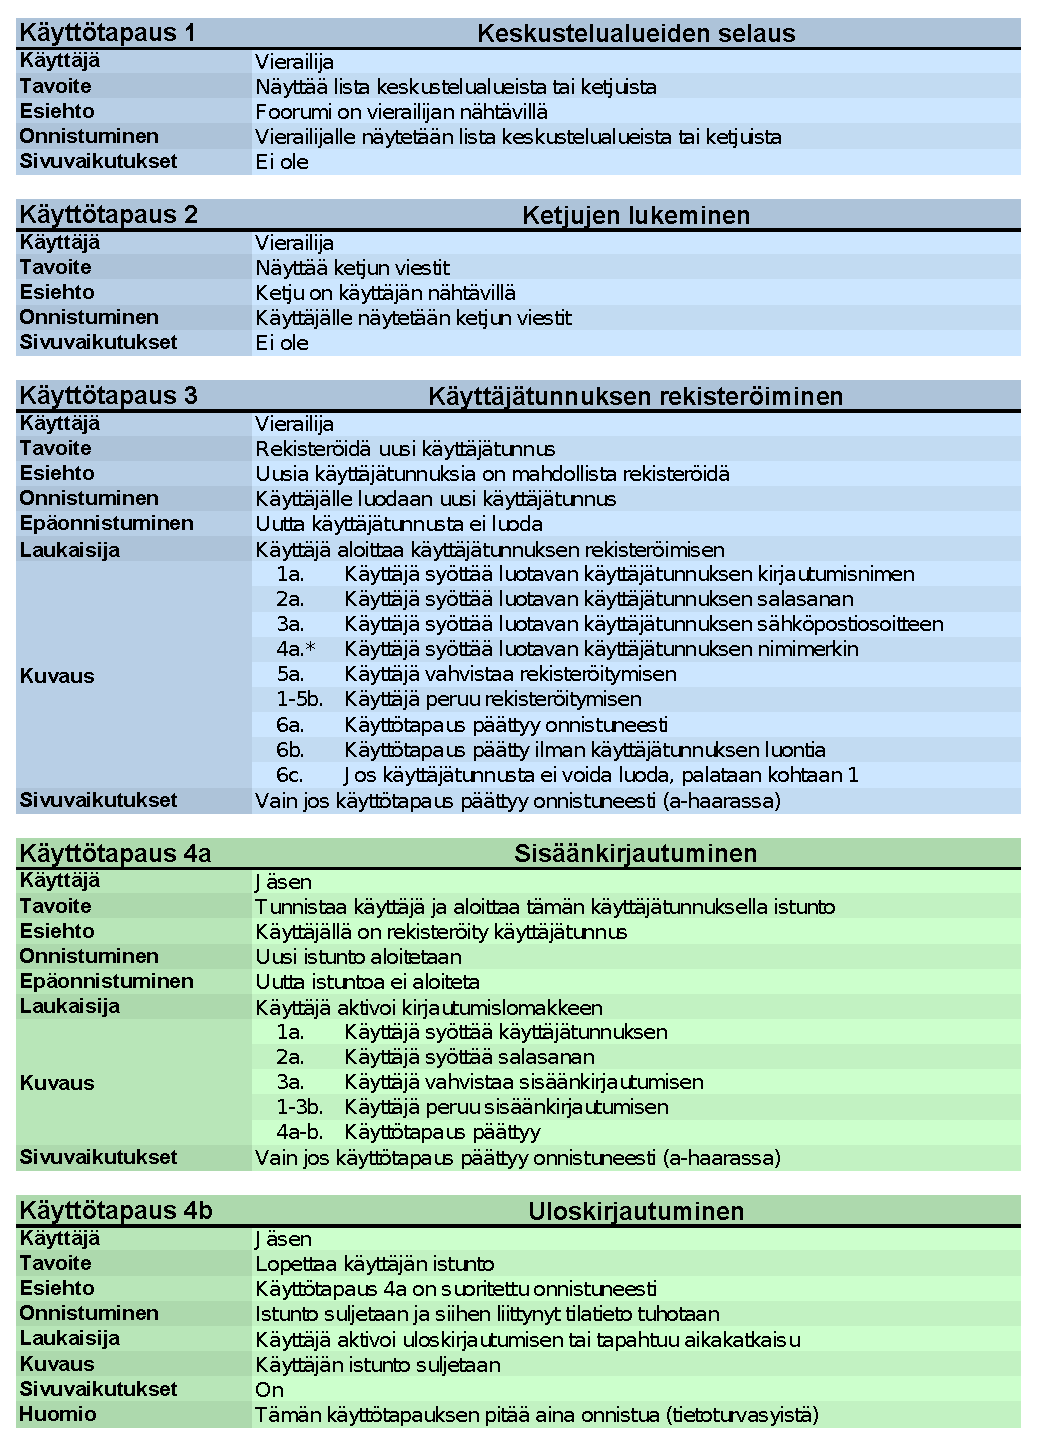
\includegraphics[trim = 27mm 0mm 0mm 25mm]{kayttotapausmalli-sivu-1.eps}\\
		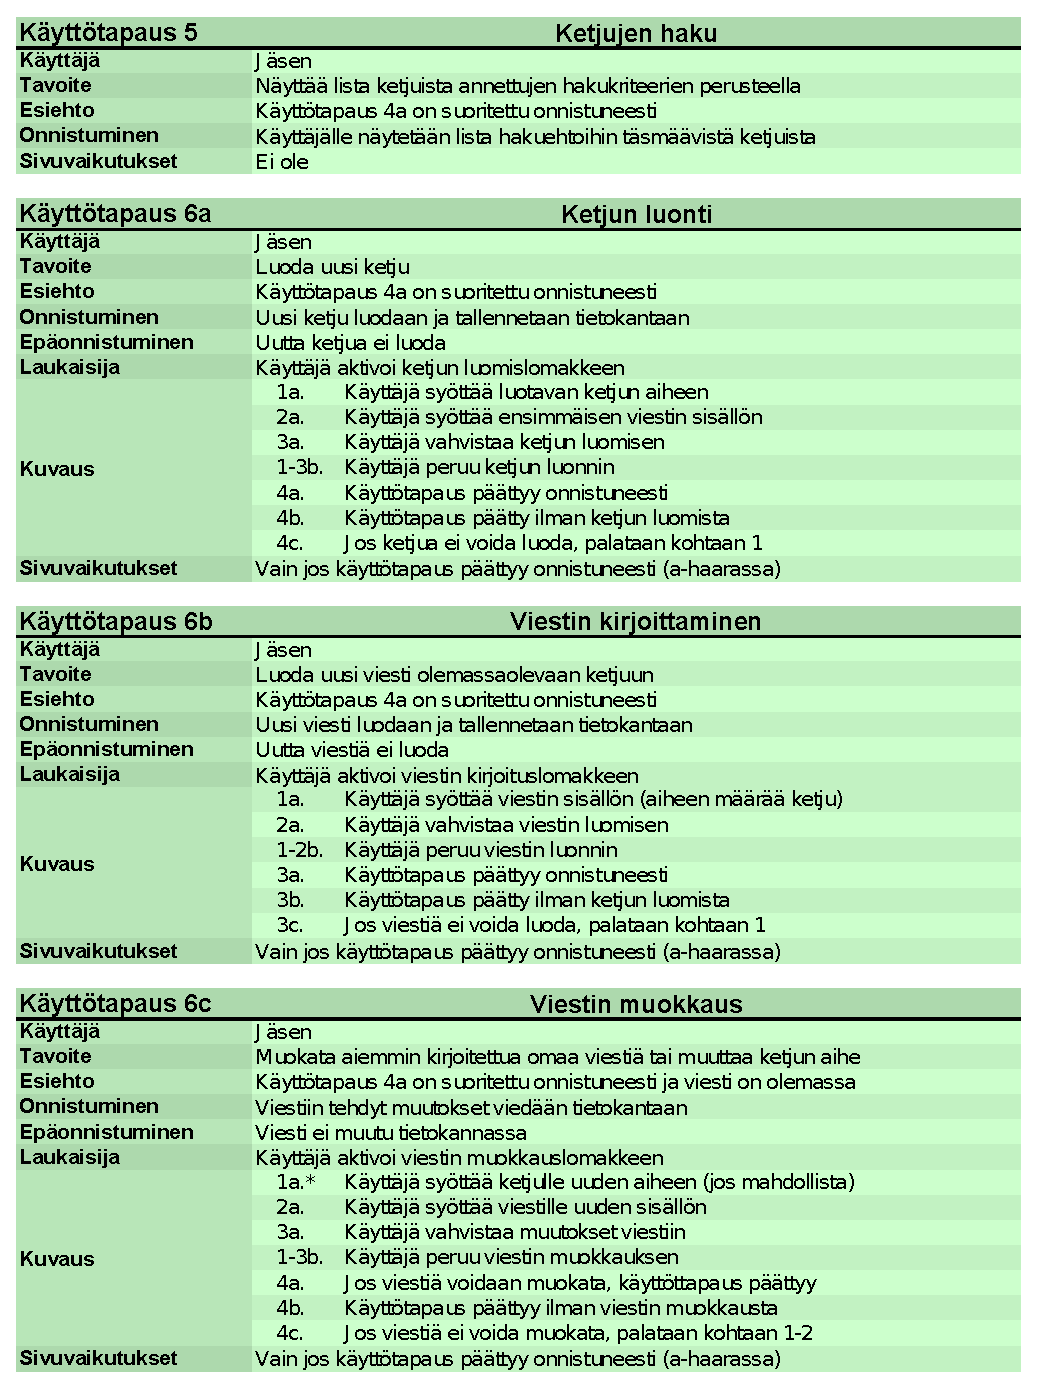
\includegraphics[trim = 21mm 0mm 0mm 25mm]{kayttotapausmalli-sivu-2.eps}\\
		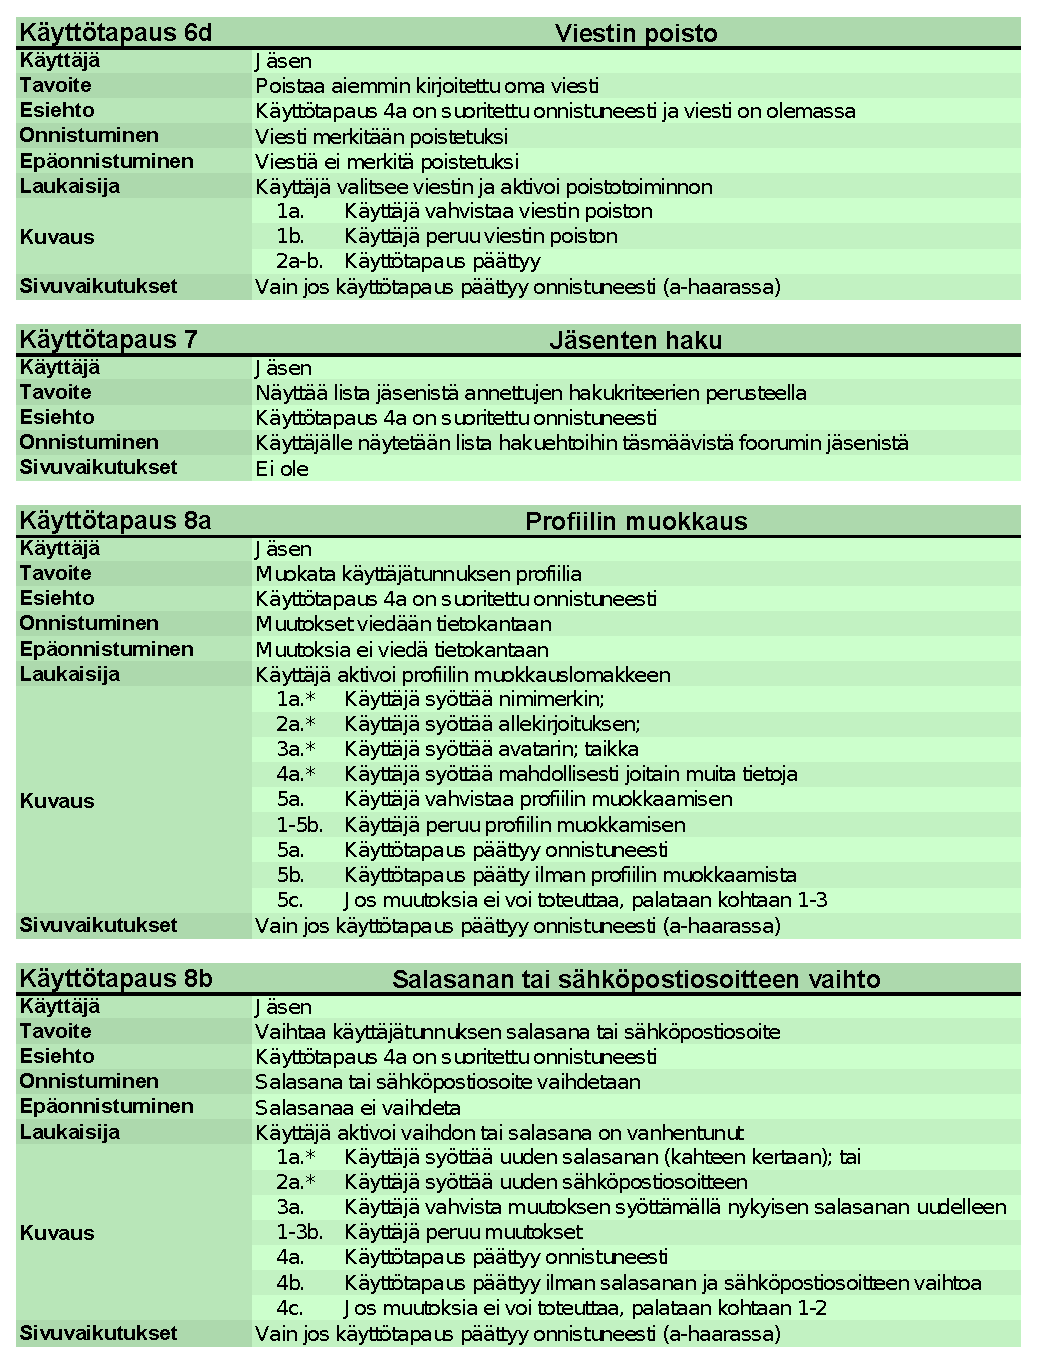
\includegraphics[trim = 21mm 0mm 0mm 25mm]{kayttotapausmalli-sivu-3.eps}\\
		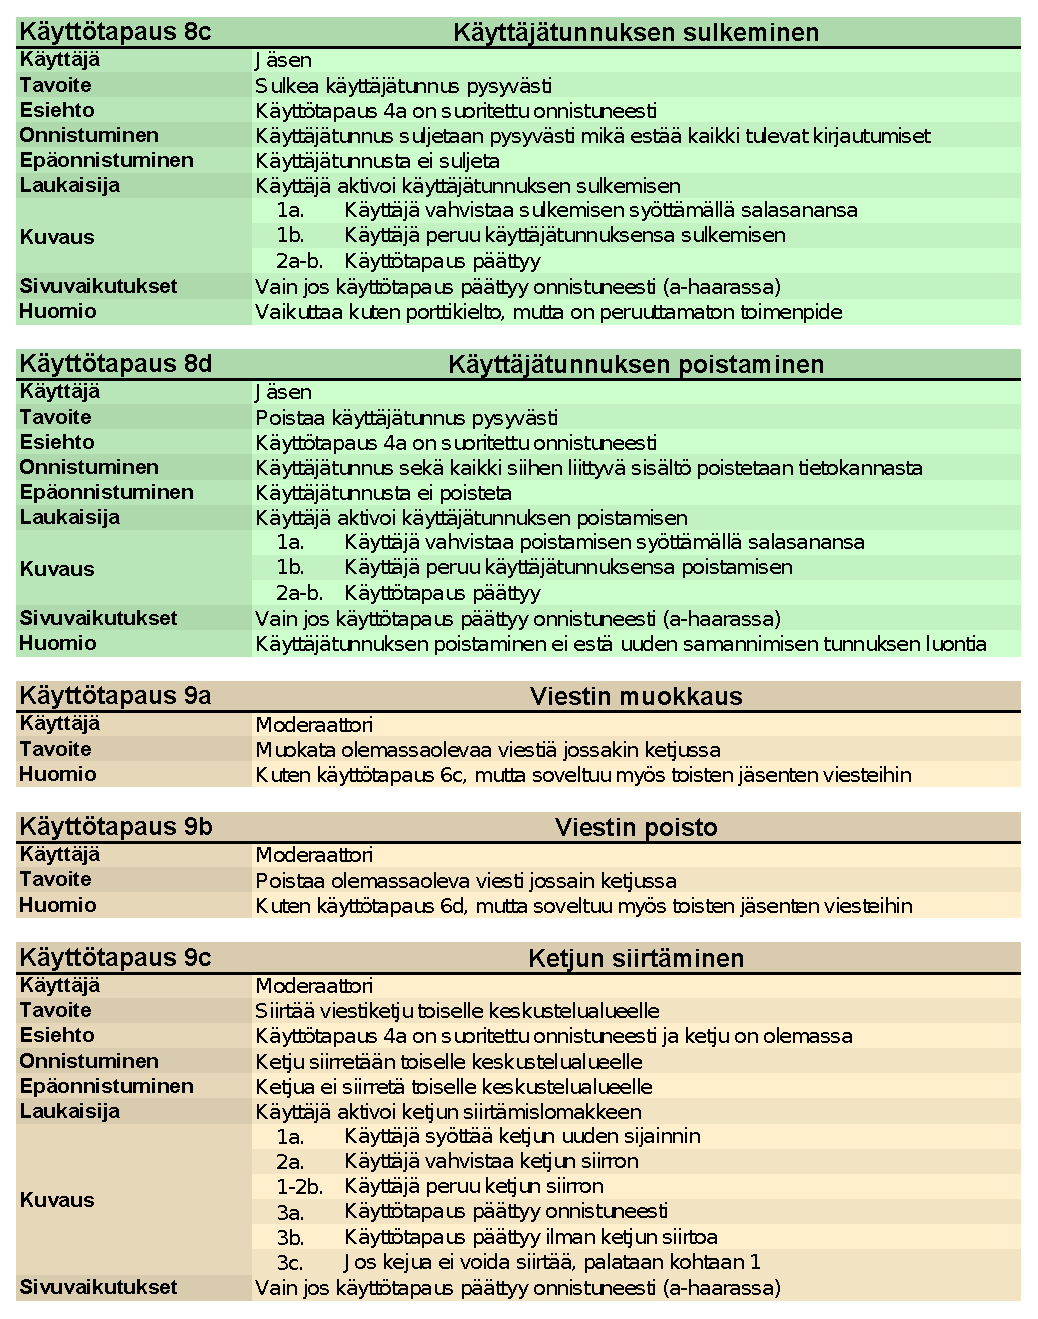
\includegraphics[trim = 21mm 0mm 0mm 25mm]{kayttotapausmalli-sivu-4.eps}\\
		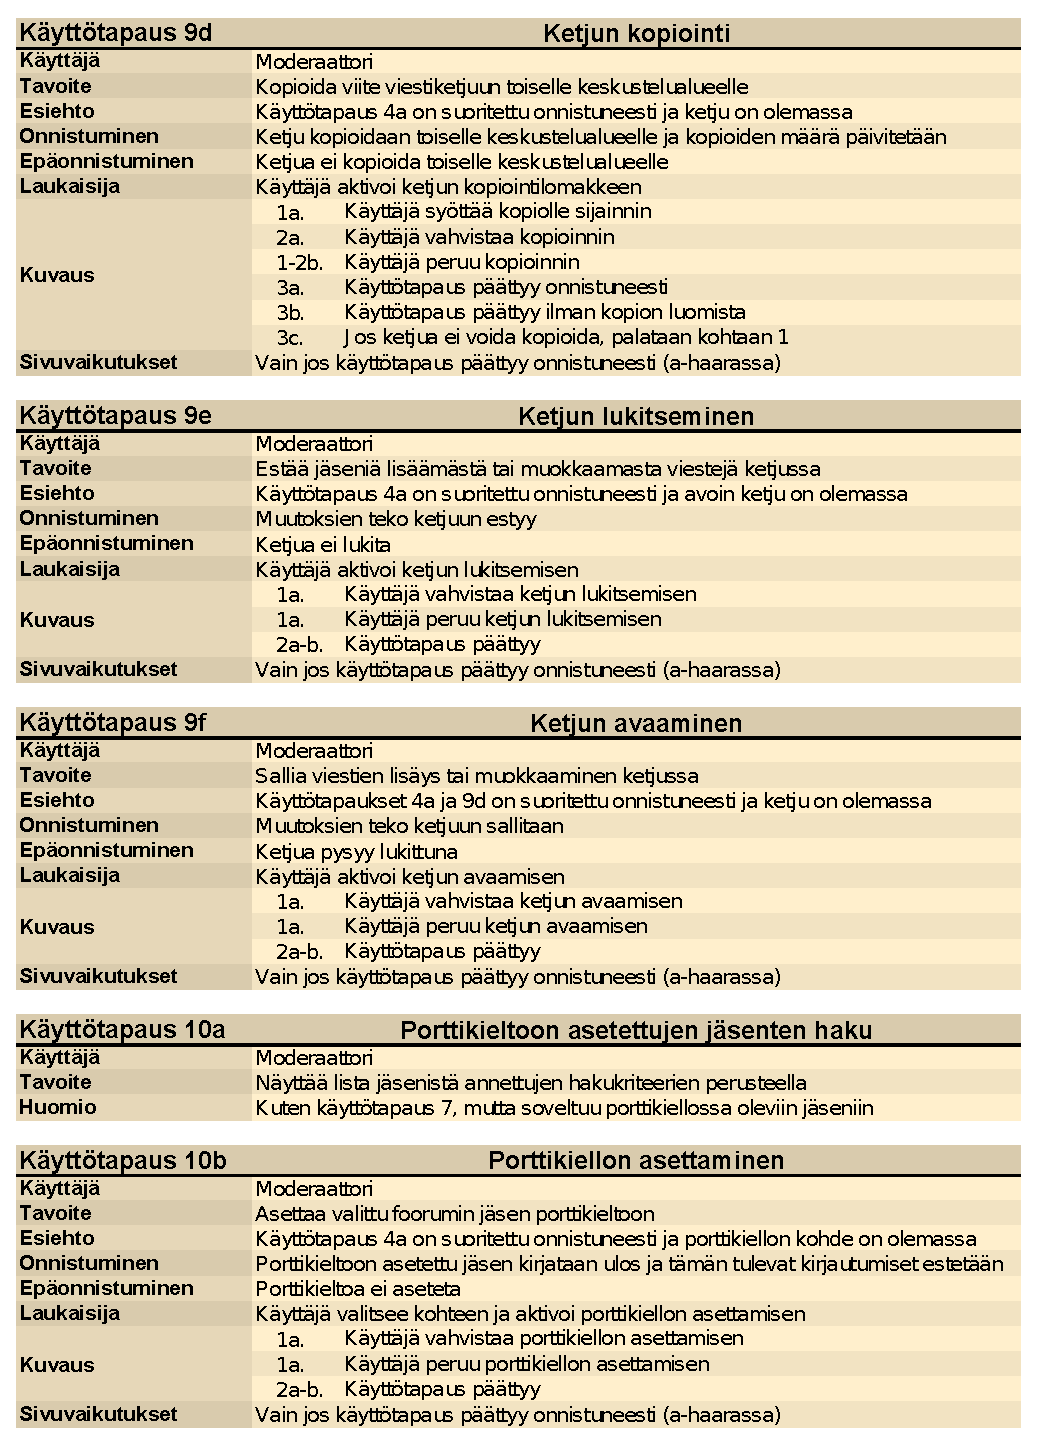
\includegraphics[trim = 21mm 0mm 0mm 25mm]{kayttotapausmalli-sivu-5.eps}\\
		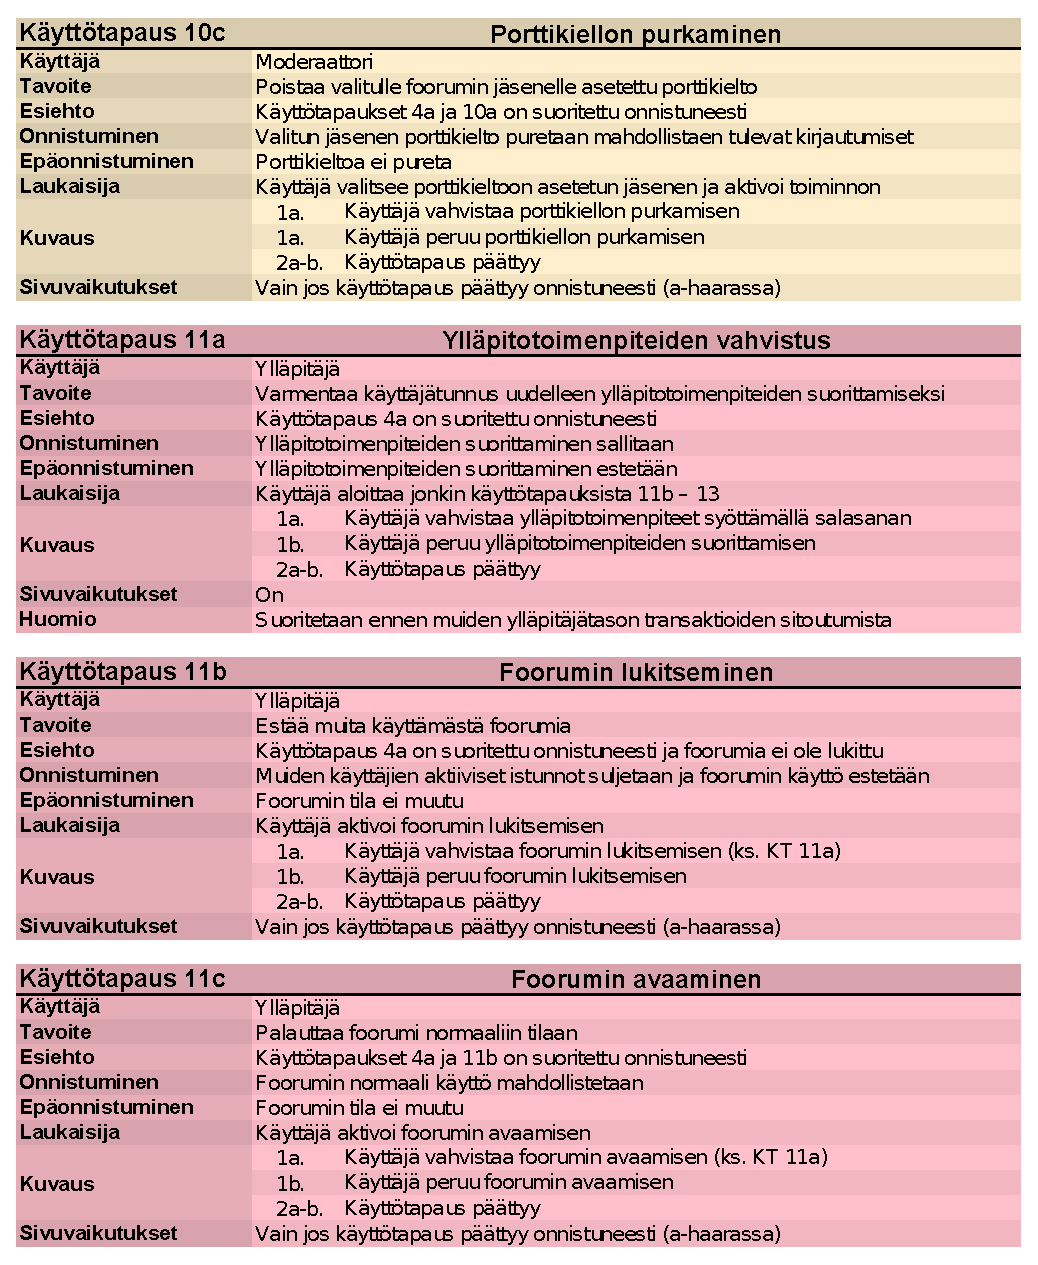
\includegraphics[trim = 21mm 0mm 0mm 25mm]{kayttotapausmalli-sivu-6.eps}\\
		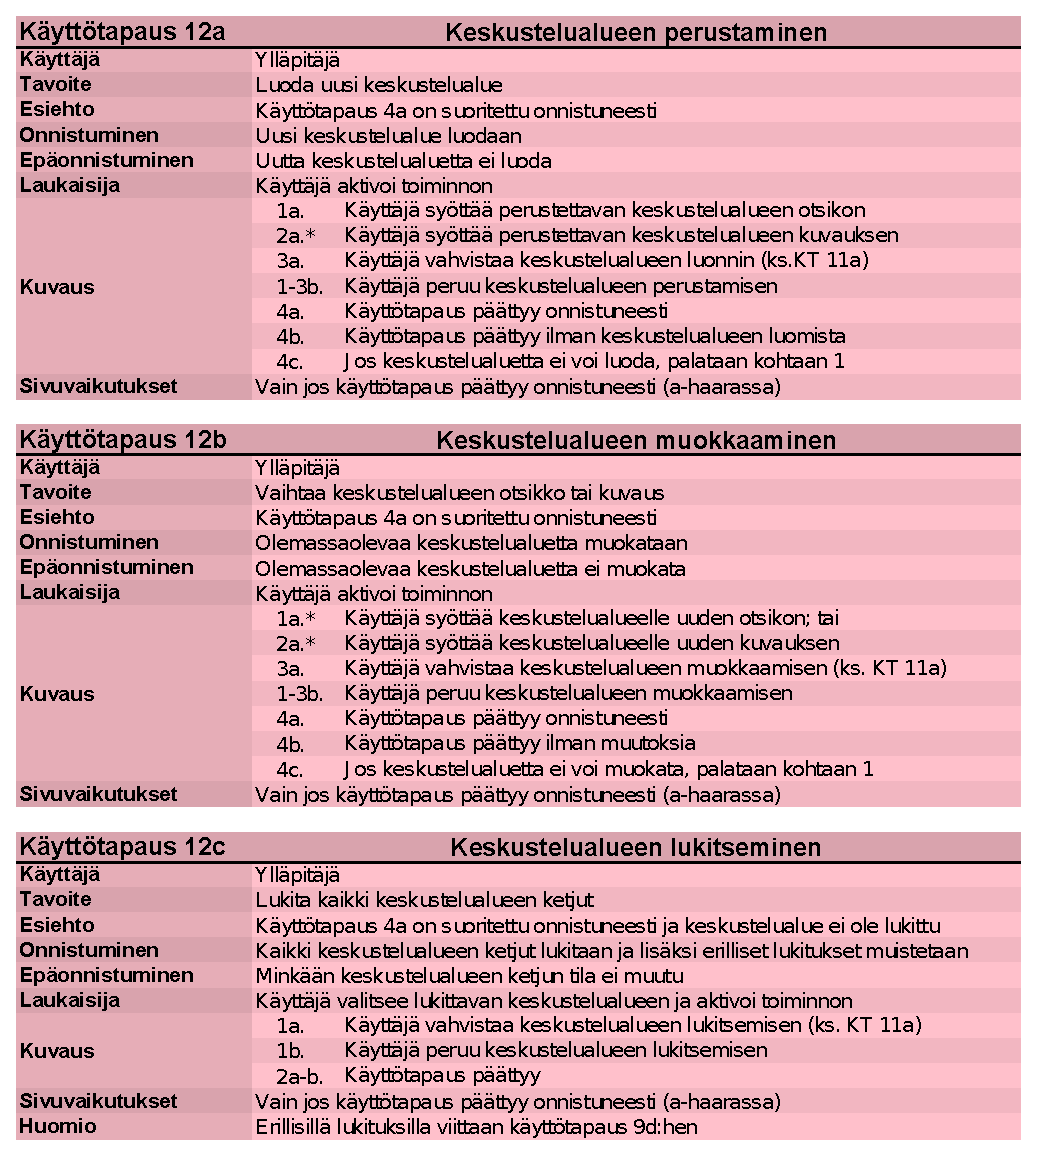
\includegraphics[trim = 21mm 0mm 0mm 25mm]{kayttotapausmalli-sivu-7.eps}\\
		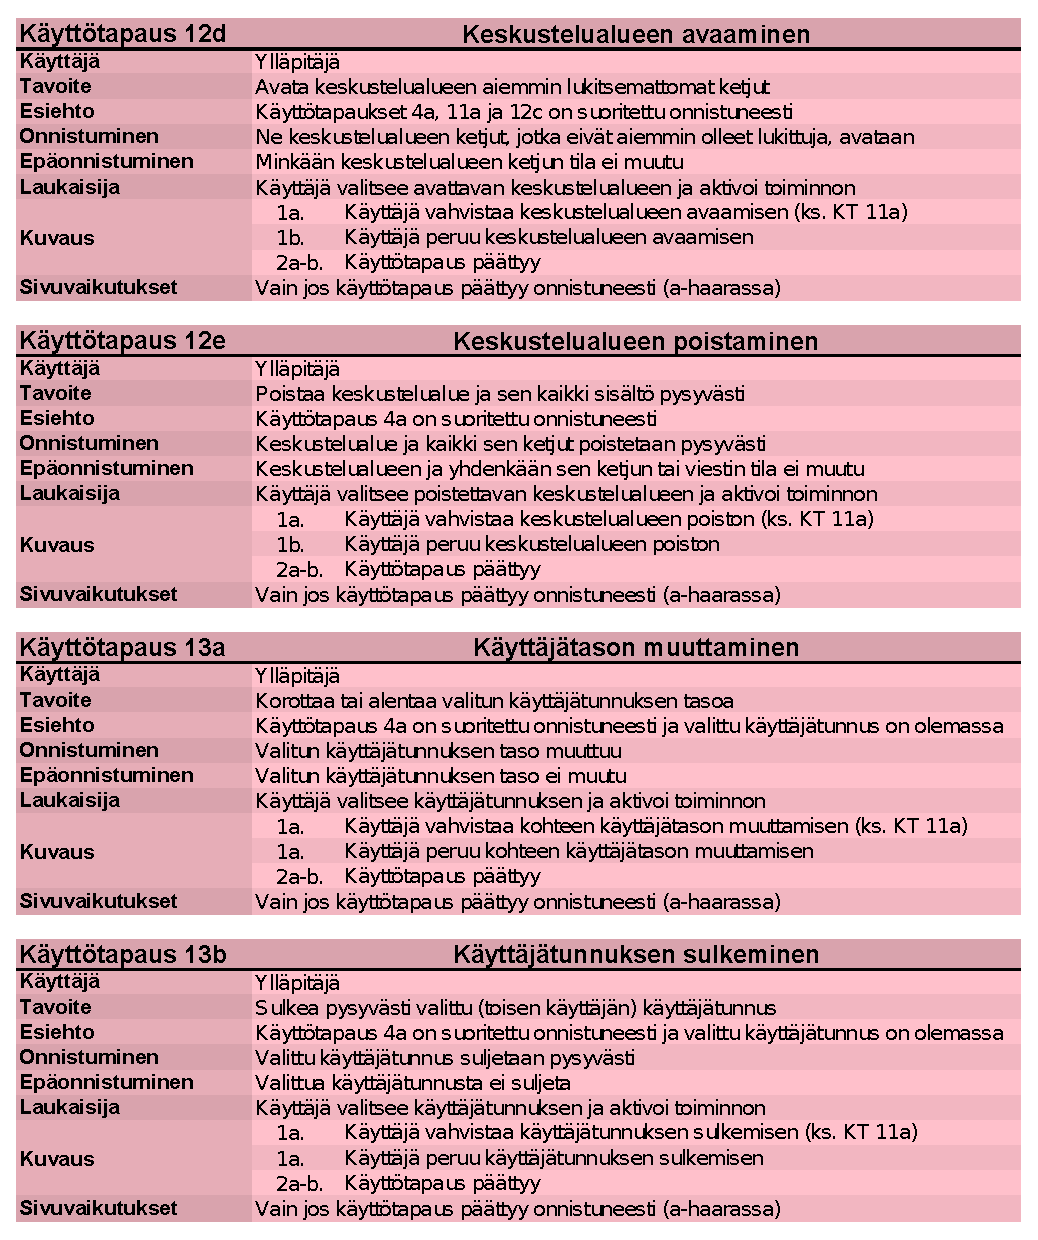
\includegraphics[trim = 21mm 0mm 0mm 25mm]{kayttotapausmalli-sivu-8.eps}\\
		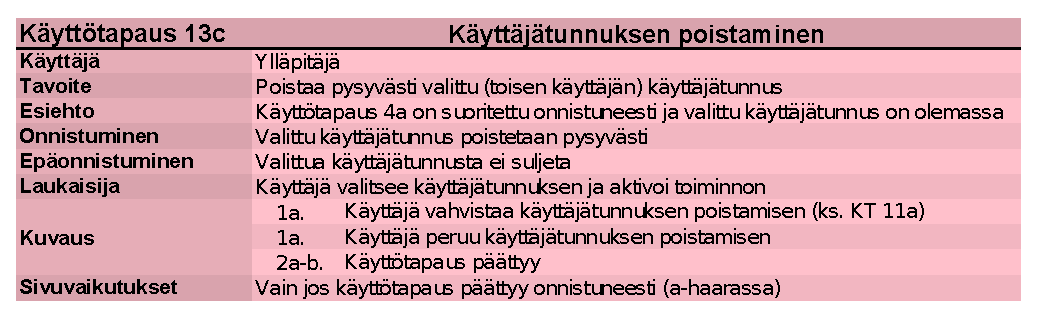
\includegraphics[trim = 21mm 0mm 0mm 25mm]{kayttotapausmalli-sivu-9.eps}\\
		
		% Ylläolevat lasken "yhdeksi" kuvaksi...
		\begin{figure}
			\caption{Käyttötapausmalli}
		\end{figure}

\newpage
\thispagestyle{plain}
\section{Tietosisältö}
	\subsection{Tietovaatimukset}
		Edellisessä kappaleessa esittämäni foorumin yleiskuvan perusteella olen päätynyt siihen tulokseen,
		että järjestelmässä on neljä tietokohdetta tai \emph{yksilötyyppiä}. Yksilötyypit ovat
		\emph{jäsen, viesti, ketju} ja \emph{keskustelualue}. Vierailijoille ei tarvita mitään tauluja
		tietokannassa sillä nämä eivät voi tuottaa sisältöä foorumille (vaikka voivatkin esimerkiksi lukea
		rajoitetusti joitakin tauluja).		
		
	\subsection{Käsitekaavio} Alla on käsitekaavio keskeisimmistä tietokohteista:
		\begin{figure}[H]		
			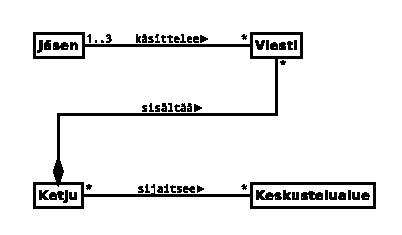
\includegraphics[trim = 0mm 0mm 0mm -3mm, scale = 2.0]{kasitekaavio.eps}
			\caption{Käsitekaavio}
		\end{figure}	
		
	\subsection{Tietokohteet} Seuraavalla sivulla olen listannut lyhyen taulukkomuotoisen kuvauksen edellä
		esi-tetyistä tietokohteista. Arvojoukolla merkkijono($n$) viittaan vaihtuvan mittaisiin korkeintaan
		$n$ merkkiä pitkiin merkkijonoihin.
	
		\newpage
		\thispagestyle{plain}
		
		\begin{figure}[H]
			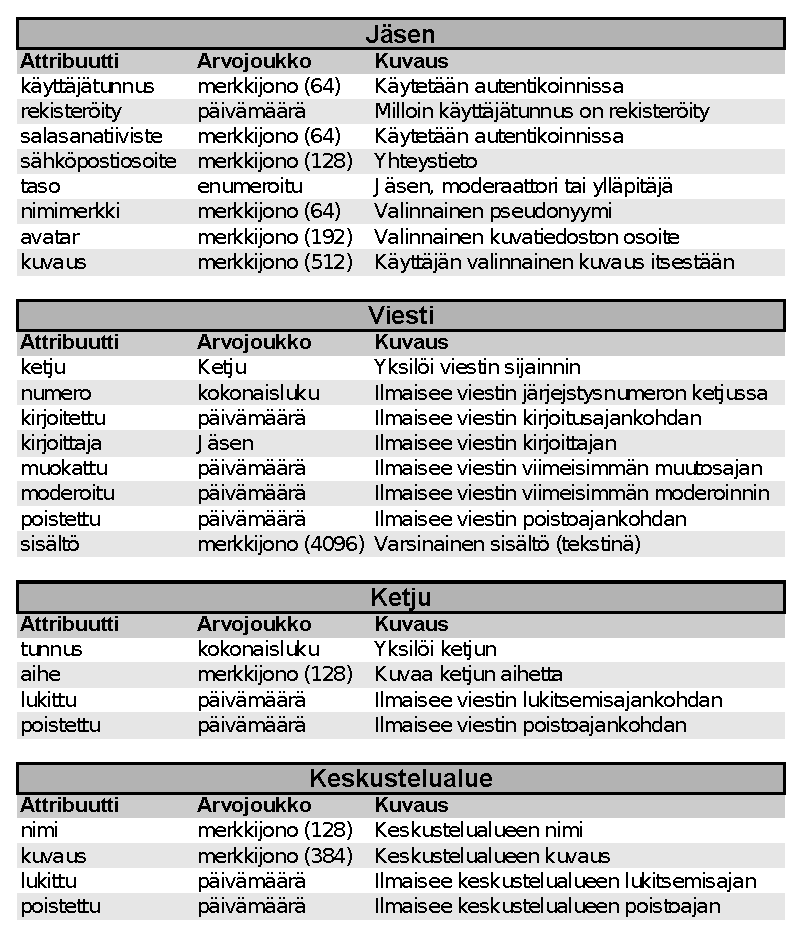
\includegraphics{tietokohteet.eps}
			\caption{Tietokohteet}
		\end{figure}
		
\newpage
\thispagestyle{plain}		
	\section{Relaatiotietokantakaaviot}
		\subsection{ER-kaavio}
			Seuraavalla sivulla on tietokannan riippuvuuksia korkealla tasolla kuvaava ER-kaavio. Olen
			esittänyt siinä kohteiden tyypit väreillä, mikä ilmenee kuvassa ole-vasta selityksestä. Lisäksi
			selvennettäköön, että olen tilan säästämiseksi niputtanut osan samankaltaisista attribuuteista 
			yhteen moniarvoisiksi attribuuteiksi (esimerkiksi salasana koostuu tiivisteestä ja suolasta,) sekä
			viitannut porttikiellon asettamiseen potkimisena. Kaikki järjestelmän todelliset tietokantataulut
			ovat vähintään kolmannessa normaalimuodossa, joten moniarvoisia attribuutteja ei tietokannassani
			esiinny.\footnote{Jostain syystä kaavioeditori on tuottanut \emph{Keskustelualueen}
			attribuuteille ylimääräisiä viivoja. Luultavasti kyseessä on bugi, joten pyydän anteeksi tätä
			esitysteknistä seikkaa (kuten myös kaamean näköistä kirjainten ladontaa joissakin taulukoissa).}
		
		\subsection{UML-kaavio}
			Olen myös laatinut tarkemman UML-tyylisen tietokantakaavion, josta ilmenee kaikki
			varsinaiseen tietokantaan luotavat taulut attribuutteineen ja avaimineen. Mainittu kaavio löytyy
			sivulta 21. Olen merkinnyt ensisijaiset ja vierasavaimet stereotyypein \flqq PK\frqq \ ja \flqq 
			FK\frqq. Lisäksi olen värittänyt taulut vaaleilla mustikan, vadelman ja banaanin väreillä siten,
			että värit korostavat lausutussa järjestyksessä varsinaisia ja epäitsenäisiä yksilötyyppejä sekä
			aputauluja.
		
		\newpage
		\thispagestyle{plain}
		\begin{figure}[H]		
			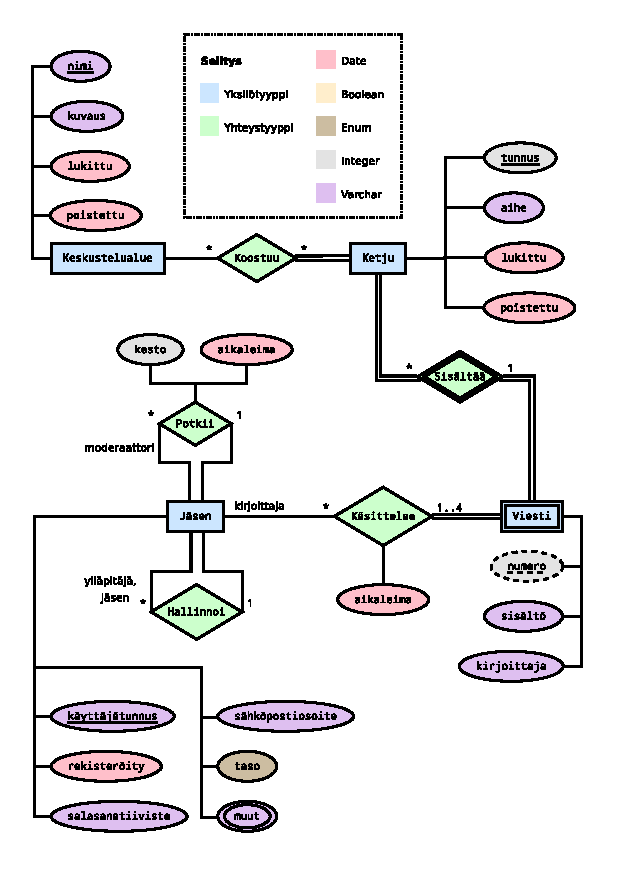
\includegraphics[trim = 6mm 0mm 0mm 20mm, scale = 1.5]{er-kaavio.eps}
			\caption{ER-kaavio}
		\end{figure}
		
		\newpage
		\thispagestyle{plain}
		\begin{figure}[H]		
			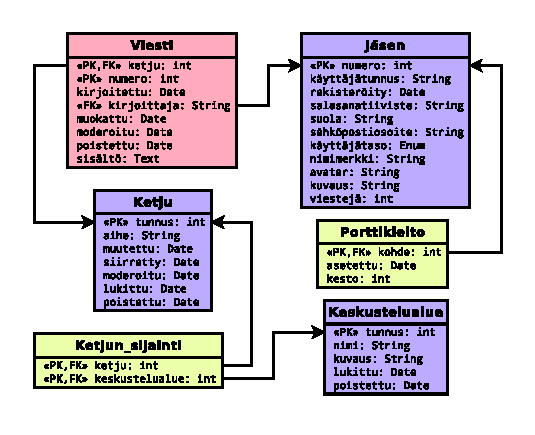
\includegraphics[trim = 0mm 0mm 0mm 20mm, scale = 1.5]{uml-tietokantakaavio.eps}
			\caption{Tietokantakaavio}
		\end{figure}
		
\newpage
\thispagestyle{plain}
	\section{Järjestelmän yleisrakenne}
		\subsection{Hakemistorakenne}
			Kuvaan tässä luvussa lyhyesti järjestelmän yleisrakennetta hakemistorakenteen muodossa.
			Projektin tärkein sisältö sijaitsee juurihakemiston alikansioissa \emph{doc}, \emph{src} ja
			\emph{web}.
	
		\subsection{Dokumentaatio}
			Hakemisto \emph{/doc} sisältää projektin dokumentaation, kuten muunmuassa tämän asiakirjan.
			\emph{/doc/src} puolestaan sisältää dokumentaation latex-lähdekoodin sekä kaaviot ja kuvat.
			
		\subsection{Kontrollerit}
			Hakemisto \emph{/src/java} sisältää projektin MVC-mallin mukaiset kontrollerit ja mallit omissa
			alihakemistoissaan. Lisäksi hakemisto sisältää foorumin käyttöönoton kannalta tarpeellisen
			konfiguraatiotiedoston omassa alihakemistossaan.
			
			\emph{/src/java/kontrollerit} sisältää varsinaisia HTTP-pyyntöjä käsittelevät servletit. Sillä on
			myös kaksi alihakemistoa:
			
			\emph{/src/java/kontrollerit/tyokalut} sisältää työkaluluokkia joiden staattisia metodeja eri
			servletit voivat käyttää. Työkaluluokkiin olen pyrkinyt keräämään yleiskäyttöi-siä koodinpätkiä
			käytettäväksi kirjastometodien tapaan.
			
			\emph{/src/java/kontrollerit/tyypit} sisältää aputyyppejä. Esimerkiksi työkaluluokka
			\emph{Listaaja} käyttää aputyyppiä \emph{ListaAlkio}, joka mallintaa web-sivuilla esitettävän
			listausnäkymän yhden rivin sisältämiä tietoja.
			
			\emph{/src/java/mallit} taas sisältää MVC-mallin mukaiset mallitiedostot. Sen alihakemistot on
			nimetty käytetyn ohjelmointikielen mukaisesti.
			
			\emph{/src/java/mallit/java} sisältää järjestelmän yksilötyyppejä mallintavat Java-luokat,
			pääsynvalvonnan peruspilarina toimivan käyttäjätunnuksen tasoa mallintavan enumeroidun luokan
			sekä Yksilötyyppien tuonnista ja viennistä vastaavan luokan \emph{TietokantaDAO}. Viimeksi
			mainittu vastaa myös useamman yksilötyypin tietokantataulujen käyttöä vaativien transaktioiden
			toteuttamisesta.
			
			Viimeisenä alihakemistona mainittakoon \emph{/src/java/mallit/sql}, joka sisältää foorumin
			ylläpidon ja käyttöönoton kannalta tärkeimmät SQL-tiedostot. Foorumin käyttöönoton yhteydessä
			tarvitaan tiedostoa \emph{Alustus.sql}.
			
		\newpage
		\thispagestyle{plain}
		\subsection{Näkymät}
			Hakemisto \emph{/web} sisältää MVC-mallin mukaiset näkymätiedostot.
			
			\emph{/web/META-INF} on foorumin käyttöönoton kannalta tärkeä hakemisto, jossa sijaitseva 
			tiedosto \emph{content.xml} sisältää tietokantayhteyden muodostamiseen tarvittavat tiedot.
			Foorumin ylläpitäjän tulee käyttöönoton yhteydessä päivittää mainittuun tiedostoon tietokannan
			sijainti, käyttäjätunnus sekä salasana.
			
			\emph{/web/WEB-INF} sisältää äsken mainitun hakemiston tavoin tiedostoja jotka eivät näy
			web-sivuja selaaville asiakkaille. Kansiossa on konfiguraatiotiedosto \emph{web.xml} sekä yksi
			alihakemisto.
			
			\emph{/web/WEB-INF/tags} sisältää kirjastoja muistuttavia tag-tiedostoja. Niitä olen
			käyttänyt toisteisuuden vähentämiseen ja koodin rakenteen selkiyttämiseen näkymätiedostoissa.
			
			\emph{/web/jsp} sisältää näkymätiedostot, jotka voivat käyttää apunaan toistuvan tiedon
			esittämiseen tag-tiedostoja.
			
			\emph{/web/tyylit} puolestaan sisältää web-sivujen graafisen tyylin määrittelystä vastaavat
			CSS-tiedostot omissa tyylien mukaisissa alihakemistoissaan. Tällä hetkellä tyylejä on vain yksi
			ja sen tiedostot löytyvät alihakemistosta \emph{oletus}.
			
			\emph{/web/data}-hakemistossa sijaitsee muita kuin koodiksi tulkittavia tiedostoja. Sillä on
			kaksi alihakemistoa:
			
			\emph{/web/data/staattinen}, joka sisältää foorumin graafisessa esityksessä tarvittavia
			kuvatiedostoja; sekä
			
			\emph{/web/data/dynaaminen}, jossa puolestaan sijaitsee käyttäjien foorumille lä-hettämät
			tiedostot joita ei katsota osaksi ohjelmistoa. Esimerkiksi käyttäjien mahdolliset avatar-kuvat
			sekä viesteihin laittamat liitetiedostot tulevat tähän hakemistoon.
			
		\subsection{Muut hakemistot}
			Muita projektikansiosta mahdollisesti löytyviä hakemistoja ovat \emph{build}, \emph{dist},
			\emph{test}, \emph{nbproject} sekä piilohakemisto \emph{.git}. Nämä hakemistot eivät 
			varsinaisesti liity tässä dokumentissa käsiteltäviin asiakokonaisuuksiin, joten katson 
			parhaaksi ohittaa niiden käyttötarkoituksen kuvailemisen. (Kyseessä on projektin tekniseen
			toteutukseen liittyviä hakemistoja, jotka lienevät Java-ohjelmoijille entuudestaan tuttuja.)
			
			Sanotusta huolimatta tahdon huomauttaa että jos projektin 
			kääntää NetBeans IDE:llä, niin .war-arkisto ilmestyy kansioon /dist. Tämä arkisto voidaan
			sijoittaa \emph{Tomcat}-palvelimen \emph{webapps}-hakemistoon.
			
		\newpage
		\thispagestyle{plain}
		\subsection{Istunto}
			Käyttäjät, joilla on käyttäjätunnus järjestelmässä, voivat kirjautua sisään erillisen lomakkeen
			kautta. Aktiivisten istuntojen hallinnoimisesta ja pääsyoikeuksien valvonnasta vastaa Java-luokka
			\emph{Valvoja}. Kirjautumisen yhteydessä käyttäjän käyttäjätunnukseen liitetään istunto lisäämällä
			näiden viitteet hajautustauluun. Vastaavasti uloskirjautumisen tai muun istunnon sulkemisen
			yhteydessä tämä avain-arvopari poistetaan hajautustaulusta. Valvoja myös tarkastaa varttitunnin
			välein onko järjestelmässä avoimia istuntoja, joissa edellisestä sivunlatauksesta on kulunut
			vähintään tunti. Kaikki tällaiset istunnot merkitään vanhentuneiksi ja poistetaan.
			
			Hajautustauluun perustuva ratkaisu tarjoaa muunmuassa seuraavat mahdollisuudet: Ensinnäkin
			järjestelmään parhaillaan sisään kirjautuneet käyttäjätun-nukset voidaan helposti listata ja laskea.
			Toisaalta myös hajautustaulun luonteesta seuraa, ettei samalla käyttäjätunnuksella voi olla useata
			samanaikaista istuntoa aktiivisena.
			
			Toisaalta on syytä pitää mielessä, ettei tämä istuntoihin liittyvä kirjanpito tapahdu tietokannan
			tasolla. Periaatteessa on mahdollista, että jos jokin taho saa tietoonsa tietokantayhteyden 
			muodostamiseen tarvittavat tiedot, voi tämä pystyttää toisen ohjelmistoani käyttävän
			foorumikäyttöliitymän ja hyödyntää tätä erilaisiin vilpillisiin tarkoituksiin. Tämän vuoksi
			on syytä pitää mielessä, ettei foorumin istuntojärjestelmä korvaa yhteyden salausta ja sertifikaatin
			käyttöä (eikä etenkään tietokannan tietojen salassapitoa).
	
\newpage
\thispagestyle{plain}
	\section{Käyttöliittymä}
		\subsection{Käyttöliittymäkaavio}
			Seuraavalla sivulla näkyvä kaavio antaa yleiskuvan käyttöliittymän komponenteista ja niiden
			välisistä suhteista. Esityksen selkeyttämiseksi olen värikoodannut komponentit niiden käyttöön
			tarvittavaa pienintä käyttäjätasoa vastaavalla väril-lä aiempaa käytäntöäni vastaavasti.
			(Toisin sanoen kaikkien käytettävissä olevat komponentit ovat sinisiä, jäsenten käytettävissä
			olevat vihreitä, moderaattoreiden keltaisia sekä ylläpitäjän punaisia.) Lisäksi on syytä pitää
			mielessä että mo-niin komponentteihin liittyy lisätoiminnallisuutta korkeammilla käyttäjätasoilla. 
			Esimerkiksi komponentti "Käyttäjätunnus" tarjoaa ylläpitäjälle palvelun, joka mahdollistaa kohteena 
			olevan käyttäjätunnuksen käyttäjätason muuttamisen.
		
		\subsection{Komponentit}
			Olen merkinnyt osaan komponenteista tiedostonimen. Nimetyssä tiedostossa on enemmän tai vähemmän
			toteutettu kyseisen komponentin toiminnallisuus.
		
			Lienee paikallaan myös hieman selventää itse komponenttien nimien merkitystä. 
			\emph{Navigointi}-komponentti muodostaa sivun kehyksen ja kaikki muut komponentit liimataan siihen
			näkymätiedostoissa. Sen avulla käyttäjä voi helposti siirtyä käyttämään tärkeimpiä toimintoja.
			\emph{Listaus} puolestaan hyödynnetään muiden komponenttien osana kirjaston tapaan. Ketjujen ja
			viestien käsittelyyn liittyvät toimenpiteet puolestaan on koottu komponenttiin \emph{Muokkaus}.
			Nämä yksilötyypit liittyvät niin läheisesti toisiinsa, että olen katsonut parhaaksi käsitellä niitä
			saman komponentin eri palvelujen kautta. \emph{Profiili} listaa joitakin rekisteröityyn
			käyttäjätunnukseen liittyviä tietoja ja sen kautta myös näiden tietojen muokkaus voitaisiin
			toteuttaa. Salasanan ja sähköpostiosoitteen vaihto sekä käyttäjätun-nuksen sulkeminen ovat niin
			merkittäviä toimenpiteitä, että niiden toteutus olisi tarkoituksenmukaisinta siirtää erilliseen
			komponenttiin \emph{Käyttäjätunnus}. Näiden, sekä ylläpitotoimenpiteiden, valtuuttaminen vaatii
			salasanan uudelleen syöttä-mistä, mistä huolehtii \emph{Vahvistus}. Sen vastuulla on myös pyytää
			heikompi tavallinen vahvistus eräille toimenpiteille.
		
			Tarkempia tietoja toteutettujen komponenttien tehtävistä ja toiminnoista löytyy Javadoc:sta.
		
		\newpage
		\thispagestyle{plain}
		\begin{figure}[H]		
			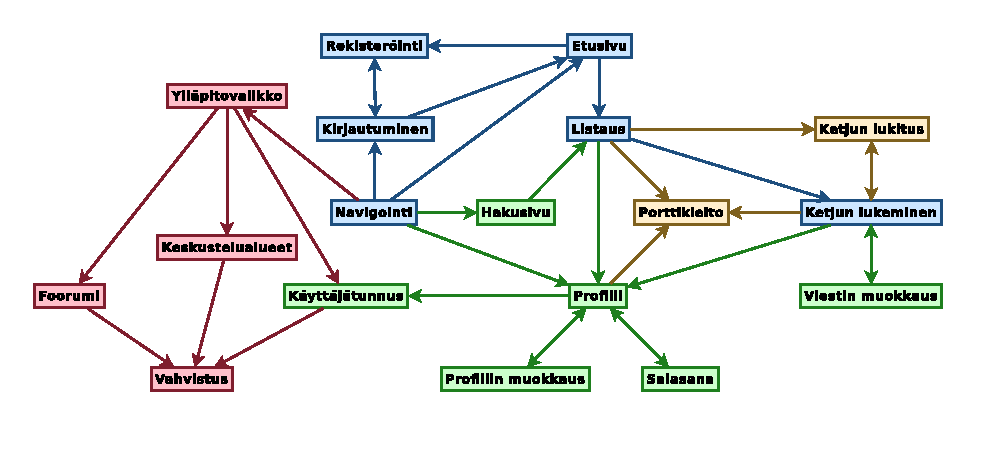
\includegraphics[trim = 12mm 0mm 0mm 0mm, scale = 1.5]{kayttoliittymakaavio.eps}
			\caption{Käyttöliittymäkaavio}
		\end{figure}
		
\newpage
\thispagestyle{plain}
	\section{Asentaminen}
		\subsection{Esivalmistelut}
			Oletan, että ylläpitäjä on tätä ohjetta lukiessaan jo asentanut \emph{Apache Tomcat 7.0.53}
			\footnote{versio 7.0.28 ei ole yhteensopiva.} (tai omalla vastuullaan uudemman) web-palvelimen
			sekä \emph{PostgreSQL}\\ -tietokannan hallintaohjelmiston sekä luonut kaikki tarvittavat
			käyttäjätunnukset.
		
			Haluan myös painottaa TLS:n tärkeyttä. Vastuullisen ylläpitäjän tulee ehdottomasti huolehtia, että
			palvelimella on validi sertifikaatti luotetulta myöntäjältä, jotta asiakkaat voivat käyttää foorumia
			(ainoastaan) HTTPS:n kautta. \emph{Ohjelmistoni ei nimittäin tarjoa minkäänlaista suojaa
			esimerkiksi salakuuntelua vastaan}, vaan olen olettanut että tuotantokäytössä liikenne asiakkaan ja
			palvelimen välillä on salattua alemmalla tasolla.
		
		\subsection{Käyttöönotto}
			Ensiksi projektikansio tai war-arkisto tulee sijoittaa palvelimen \emph{webapps}-hakemis-toon.
			Oletan seuraavaksi, että ylläpitäjä on siirtynyt komentotulkissa projektikansion juureen.
		
			Kun hakemistorakenne on luotu, tulee suorittaa tietokantataulut määrittelevä SQL-tiedosto komennolla
			\emph{psql src/java/mallit/sql/Alustus.sql}.\footnote{Tilanteesta riippuen saattaa olla
			tarpeellista määrittää esimerkiksi käyttäjä, tietokannan nimi sekä salasana asianmukaisin lipuin,
			joiden käyttöohjeet löytyvät psql:n manuaalista.}
		
			Seuraavaksi tulee tietokantayhteyden muodostamiseen tarvittavat tiedot täyt-tää tiedostoon
			\emph{web/META-inf/context.xml.dist} ja poistaa sen nimen perästä .dist-pääte. Kyseisessä
			tiedostossa on mainittu kommentissa mitä tietoja tulee täydentää. 
		
			Tässä vaiheessa mainittakoon, että koska en kyennyt erinäisten vastoinkäy-misten vuoksi täysin
			noudattamaan aikataulua, jäi muunmuassa keskustelualueiden muokkaustoiminnot toteuttamatta.
			Tällä hetkellä keskustelualueet pitää lisätä käsin tietokantaan SQL-kyselyllä "\texttt{insert into
			alueet (nimi, kuvaus)\\ values ('\flq nimi\frq', '\flq kuvaus\frq');}", missä \flq nimi\frq
			\ tulee korvata lisättävän alueen nimellä ja \flq kuvaus\frq \ kuvauksella. Kysely voidaan
			suorittaa interaktiivisessa komentotulkissa.
		
			Kun kaikki nämä toimenpiteet on onnistuneesti suoritettu, on foorumi valmis käytettäväksi ja sivun
			voi avata yleisölle.
		
\newpage
\thispagestyle{plain}
	\section{Käyttöohje}
		\subsection{Esimerkkidata}
			Foorumin toimintoja pääsee helposti testaamaan suorittamalla (vasta-alustetussa tietokannassa)
			psql-komentotulkilla kansiossa \emph{src/java/mallit/sql} sijaitseva tiedosto
			\emph{Esimerkkidata.sql}. Kyseisen tiedoston sisältämät \emph{insert}-lauseet lisäävät
			tietokantaan neljä keskustelualuetta sekä neljä käyttäjätunnusta.
		
			Käyttäjätunnukset ovat \emph{maija} (ylläpitäjä) salasanalla \emph{salasana}, \emph{esmer}
			(moderaattori) salasanalla \emph{1234}, \emph{mattimeik} salasanalla \emph{abcdef} sekä tRolli
			(pysyvässä porttikiellossa) salasanalla \emph{lällispöö}.
		
		\subsection{Esimerkkipalvelin}
			Yllämainitut käyttäjätunnukset toimivat myös esimerkkipalvelimellani, jonka osoi-te on
			\emph{http://91.158.178.74:8080/tsoha/}.
			
		
		\subsection{Ylläpito}
			Vaikka foorumin ominaisuuksista onkin tällä hetkellä varmasti yli puolet toteuttamatta, on
			kaikkein välttämättömin osa niistä toteutettu.
			
			Keskustelualueiden ja käyttäjätunnusten muokkaamiseen sen sijaan tarvitaan (onneksi melko
			yksinkertaisia) SQL-kyselyjä, joita en kuitenkaan tässä ohjeessa käsittele.
			
			Joka tapauksessa haluan kuitenkin mainita, että foorumin saa tyhjennettyä viesteistä suorittamalla
			SQL-tiedoston \emph{ViestienTuhoaminen.sql}. Kaikki tietokantataulut saa poistettua suorittamalla
			tiedoston \emph{FooruminTuhoaminen.sql}. Nämä löytyvät samasta hakemistosta kuin aiemmin
			asennusohjeessa mainitsemani Alustus.sql.			
		
\newpage
\thispagestyle{plain}

	\section{Tunnetut bugit, puutteet ja kehitysideat}
		\subsection{Testauksesta}
			En ohjelmoinut tällä kurssilla yksikkötestejä, vaan testasin ominaisuuksia jatkuvasti sitä mukaa
			kun niitä toteutin. Lisäksi sain nauttia runsaasta debuggauksesta NetBeansilla ja Firefoxilla.
			
		\subsection{Tunnetut bugit}
			Vaikka sainkin toteutettua ketjujen poistotoiminnon, en ehtinyt toteuttaa jäsen-ten kirjoittamien
			viestien lukumäärien päivitystä samassa yhteydessä. Toisin sanoen kokonaisen ketjun poistaminen
			aiheuttaa sen, että kaikilla siihen osal-listuneilla jäsenillä jää kirjatuksi todellista suurempi
			viestien määrä. Lisäksi ketjun (tai alueen) poistaminen ei poista heti siihen mahdollisesti
			etusivulla osoittavaa linkkiä, sillä etusivu päivitetään korkeintaan viiden minuutin välein. En
			kuitenkaan pidä tätä bugina (vaikka olisi toki mahdollista toteuttaa tällaisia tilanteita varten
			joku mekanismi etusivun päivityksen pakottamiseksi). Myös etusivun päivitysväliä voisi ehkä
			tiivistää esimerkiksi minuuttiin.
			
		\subsection{Kehitettävää}
			Puuttuvia ominaisuuksia suorastaan on vaikka millä mitalla, joten en ala niitä listaamaan tässä.
			Sen sijaan haluan todeta, että johtuen tietokannan rakenteesta, erilaisten uusien ominaisuuksien
			ja kyselyiden lisääminen on nähdäkseni melko helppo tehtävä. Redundanssia tauluissa ei paljoa
			esiinny; mieleen tulevat lähinnä jäsenen ja viestin numerot, ketjun muutosaikaleima
			sekä jäsenen viestien määrä.
		
\newpage
\thispagestyle{plain}
	\section{Omat kokemukset}
		Opin tällä kurssilla, että (web-pohjaisen) tietokantasovelluksen tekemisessä\\ ainoa helppo asia itse
		asiassa on varsinainen tietokannan käyttö, vaikkakin JDBC:n rajapinta oli mielestäni hieman...
		erikoinen.
	
		Lisäksi opin, että uusien työkalujen ja tekniikoiden opettelu vie aikansa, mikä on syytä huomioida
		projektin aikataulutuksessa. Tunsin vasta neljännellä viikolla joten kuten päässeeni kiinni
		JSP-maailmaan. Luulen tosin, että Tomcat:lla debuggaus on taito, jonka oppimiseksi täytyisi käydä
		vähintään itse tämän kurssin laajuinen pohjustus. Jatkossa ehkä osaan hieman paremmin olla valitsematta
		entuudestaan tuntemattomia välineitä ja noudattaa ohjeita kirjaimellisemmin.
		
		Huomasin myös, että olio-ohjelmoinnin ja relaatiotietokantojen risteyskoh-dissa esiintyy
		mielenkiintoista ongelmanasettelua, johon en omassa sovelluksessani keksinyt kovin tyylikästä
		ratkaisua. Käyttämäni DAO:hin ja tehdasmetodeihin perustuva mallinnustapa nimittäin tuottaa paljon
		ikävää toisteisuutta mallien koodiin. Olio-relaatio-kuvauksiin olisi mukava hieman perehtyä jatkossa. 
		
		Kaiken kaikkiaan koen että kurssi tarjoaa melkoisen määrän pureskeltavaa ja olisin kovin kiinnostunut
		näkemään oikeasti kuudessa viikossa yhden hengen toteuttaman foorumin. Tämän kurssin kävijät saavat
		totisesti noppansa ansaita!
\newpage
\thispagestyle{plain}
\listoffigures

\newpage
\thispagestyle{plain}
	\begin{thebibliography}{9}
			
		\bibitem{a}
			Defuse Security,
			\emph{Secure Salted Password Hashing}, 2014. Artikkeli ja alkuperäinen lähdekoodi: 
			https://crackstation.net/hashing-security.htm
			
		\bibitem{b}
			Alex Sirota,
			\emph{Ultimate CSS Gradient Generator}, 2014. Web-sivu:\\  
			http://www.colorzilla.com/gradient-editor/
	
		\bibitem{c}
			Alistair Cockburn,
			\emph{Basic Use Case Template}, 1998. Ladattu osoitteesta:\\ http://www.cs.helsinki.fi/u/mluukkai/ohmas10/usecase.pdf
	
	\end{thebibliography}
	
\end{document}